\section{ROBOT MOTION PLANNING}

\label{sec:motion-planning}

To design a motion planning method that minimizes psychological discomfort when a flapping drone approaches a human, we must consider the several factors:

\subsection{Distance}
\label{sec:distance}
Given the expected size and shape of a flapping drone, we estimate that the minimum acceptable distance falls within a specific range. By maintaining this distance while gradually invading the landing zone, the psychological safety can be ensured.
Several studies have investigated the psychological burden imposed by drones depending on their distance from humans useing different drone sizes\cite{Yeh2017Proxemics, lieser2021evaluating-distances,Duncan2013comfortable-approach, Acharya2017robot-vs-drone-comfort}.
Lieser et al. \cite{lieser2021evaluating-distances} focuses on tactile drone interaction using a drone with a wheelbase of 0.92m, which is suitable for palm landing.
This work conducted an experiment in which participants were asked to stop the drone when they felt uncomfortable by using foot (non-contact) and hand (contact) methods.
The results show that the maximum stop distance was approximately 1.25m,
which means that, if the drone needs to approach closer than this distance, it should be done in psychologically safe manners such as gradually decreasing the speed or using a trajectory that does not directly approach the user so that the user does not feel threatened.

Moreover, the study \cite{lieser2021evaluating-distances} also shows that even the minimum stop distance was above 0.30m, 
which means that the drone should not approach the user closer than this distance.
This indicates that physical contact should occur outside this range to guarantee physical and psychological safety.

Additionally, the front side of the drone should be always directed towards the chest of the user
because then that will prevent the wings from invading further into the user's personal space.

\subsection{Altitude}

In the study \cite{lieser2021evaluating-distances}, the height was set to enable a convenient way of tactile interaction 
by allowing the participants to slightly look down to the quadrotor.
We follow this setting because then users do not need to move their head to look up to the drone and are able to simultaneously observe both the drone and their own hand, 
which leads to easier adjustmunts of the hand position while the drone is approaching.
Assuming that users lift their hand to the height of their elbow for palm landing, the drone should be positioned at the height of between the elbow and the eye level.

\subsection{Approach Direction}

As noted in \cite{lieser2021evaluating-distances}, the approach direction of the drone affects the psychological burden.
The study shows that the participants felt most uncomfortable when the drone approached them from the back because they could not see the drone.
Therefore, the drone should approach the user from the front or side to minimize the psychological burden.


\subsection{Velocity}

KleinHeerenbrink et al. \cite{kleinheerenbrink2022optimization} showed that, in actual bird perching behavior, birds postpone stall until they were as close to the perch as possible.
However, this approach method might not be suitable for drones because the sudden deceleration might threat the user's psychological safety.
To assess the appropriate velocity of the drone, we need to consider the human perception of speed of an approaching object.
Kolling et al. \cite{Kolling2012weber-fechner-law} shows that the drivers' perception of the speed of an foregoing vehicle follows Weber's Law:

\begin{equation}
    k{\frac{\Delta {\rm W}}{W}}=\Delta s
\end{equation}

where $W$ is the measurable stimuli, $s$ the intensity of sensation, $\Delta$ the increment of physical quantity ($W$) and sensation intensity ($s$), and $k$ the coefficient. 
In the study \cite{Kolling2012weber-fechner-law}, $W$ corresponds to the the distance between the cars and $s$ to the speed of the driver's car.
We assume that the same law can be applied to the perception of the speed of an approaching drone by regarding the distance between the drone and the user as $W$ and the perceptive distance from the drone as $s$.
This assumption explanes the result of the previous study on perceived safety of drones \cite{van2023perceived-safety}, 
which shows the trend that larger distances are perceived as overly safe while a fast-moving drone close to participants is perceived as less safe than needed,
because we can consider from the law that the participants perceive the speed of the drone as too slow due to the large distance between the drone and the participants and as too fast due to the short distance between the drone and the participants.
Denoting the speed of the drone as $v$, the distance between the drone and the user as $d$, and time as $t$, we can derive the following equation:

\begin{equation}
    \label{eq:weber}
    k{\frac{\Delta d}{d}} = k{\frac{v\Delta t}{d}}=\Delta s
\end{equation}
To secure the psychological safety, the drone should approach the user keeping $\Delta s$ constant.
Denoting $k^\prime = {\Delta s/k}$, the speed can be caliculated as follows:

\begin{equation}
    v = {\frac{k^\prime d}{\Delta t}}
    \label{eq:speed}
\end{equation}
where $k^\prime$ is a constant.
In actual applicatoins, $\Delta t$ is a short time interval at which the drone changes its speed, 
which we set to 0.1s in the present study.
The distance $d$ ranges from 0.30m to 1.25m as described in \ref{sec:distance}.
In the study \cite{lieser2021evaluating-distances}, the maximum speed of the drone was set to below 1.0m/s.
Therefore, we can calculate the range of $k^\prime$ as $k^\prime \le 0.33$.  
We let $k^\prime = 0.2$ to fit this range at a large distance from the user.
Then, the one-dimentional goal position $P(t)$ which the drone should reach at time $t$ can be calculated as follows:
\begin{equation}
    \begin{aligned}    
        P(t) &= P_c(t-\Delta t) + v\Delta t = P_c(t-\Delta t) + k^\prime d\\
    \label{eq:goal}
    \end{aligned}
\end{equation}
where $P_c(t)$ is the current position of the drone.
For sufficiently large $t$, on the assumption that $d$ converges to 0, $P_c(t)$ consides with $P(t)$. 
We use this equation to send the goal position $P(t)$ to the drone at each time step of $\Delta t$.

\subsection{Trajectory Design}
\label{sec:trajectory}

\begin{figure}[t]
    \centering
    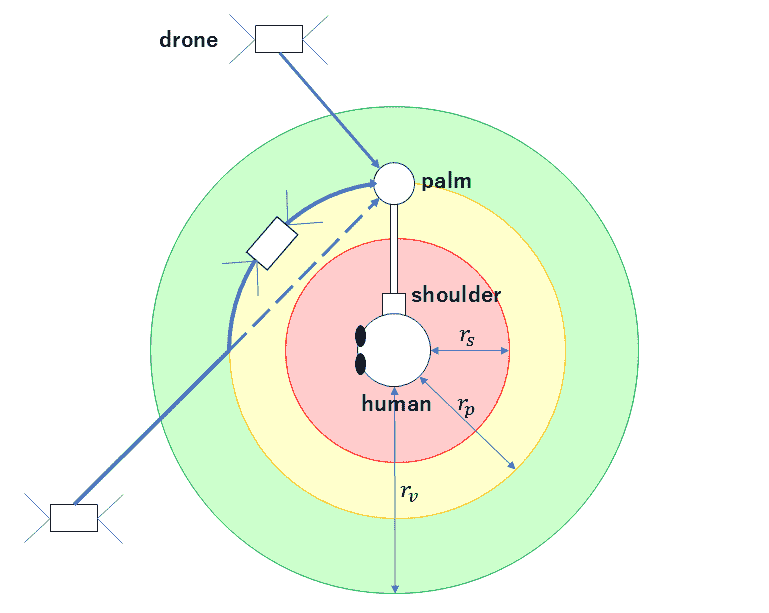
\includegraphics[width=\columnwidth]{motion-planning.png}
    \caption{Proposed motion planning for flapping drone approach. It has 4 domains which are separated by the distance from the user. Different strategies are applied to drone motion in different domains.
    }
    \label{fig:trajectory}
\end{figure}

Based on the above assumptions, we propose the following motion planning method, as illustrated in Figure \ref{fig:trajectory}.
We divide the approach trajectory into four domains based on the distance between the drone and the user $r$.

\begin{enumerate}
    \item $r > r_v$
    
    The drone is far from the user and approaches the palm straight at a constant speed.
    We let $r_v$ = 1.25 based on Section.~\ref{sec:distance}.

    \item $r_v \geq r > r_p$
    
    The drone is close enough to the user to be possibly perceived as unsafe, 
    so it determines the goal position based on Eq.~(\ref{eq:goal}) with $k^\prime = 0.2$.
    However, in actual applications, we find that the drone becomes too slow at a short distance from the user.
    To avoid this, we change $k^\prime$ from 0.2 to 0.5 at a distance of 0.3m from the palm.

    \item $r_p \geq r > r_s$
    
    The drone is inside the circle with the radius of user's arm length $r_p$ centered at the user's chest.
    To maintain a certain distance from the user, the drone moves along the circle toward the user's palm while decelearting.
    On this path, the velocity of the drone towards the user's chest is always zero,
    which means $\Delta s$ = 0 in (\ref{eq:speed}) and minimizes the threat to the perceived safety.

    \item $r \leq r_s$
    \label{sec:innermost}
    
    If the palm is within this range, the drone stays still and waits for the user to move their palm to the landing position outside the range so that the drone will not intrude the domain.
    We let $r_s$ = 0.30m based on \ref{sec:distance}.

\end{enumerate}